\chapter{Functional Data Structures}
\label{fds}
A data structure is purely functional if it supports only
non-destructive updates. These data structures are persistent, which is
especially advantageous when dealing with multiple versions of the same
object. This chapter describes the functional data structure implemented
for this thesis.

\section{Purely Functional Data Structures}

In imperative data structures, only one version of the data structure is
available. An update on an imperative data structure destroys the
previous version. Such updates are therefore known as destructive
updates. In contrast, functional data structures support only
nondestructive updates, which preserves both the old and new version of
the data structure for further processing. The data structures that
preserve their previous version when they are modified are said to be
persistent. Figure~\ref{desup} and Figure~\ref{nondesup} respectively
demonstrate destructive and nondestructive update on the binary tree
from Figure~\ref{tree}.

%Persistence is a
%property of functional languages and this property of the language makes
%the data structures persistent. 

%,
%i.e. each modification creates a new version of a data structure and the
%old one is also preserved

%The property of
%persistence makes functional data structures flexible.


\begin{figure} [htb]
  \centering
  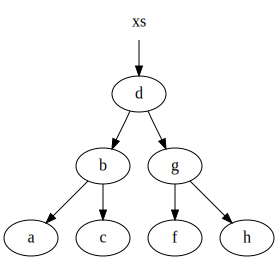
\includegraphics[scale=0.16]{tree.epsi}
  \caption{A Binary Tree}
  \label{tree}
\end{figure}


\begin{figure}[ht]
  \begin{adjustwidth}{-2em}{}
  \begin{minipage}[b]{0.5\linewidth}
    \centering
    \includegraphics[scale=0.6]{desup.epsi}
    \caption{Destructive Update}
    \label{desup}
  \end{minipage}
  \hspace{0.6cm}
  \begin{minipage}[b]{0.5\linewidth}
    \centering
    \includegraphics[scale=0.6]{nondes.epsi}
    \caption{Nondestructive Update}
    \label{nondesup}
  \end{minipage}
  \end{adjustwidth}
\end{figure}

The property of persistence makes purely functional data structures the
right choice for the applications that need to maintain multiple
versions of the data structure especially to support programming in
functional style and immutability in these data structures makes it
easier to reason about the parallelism in programs. Operations on purely
functional data structure can be performed in parallel because there are
no side effects changing the data structure.

%The applications which need to maintain multiple versions of the data
%structure 

%\begin{figure} [htb]
%  \centering
%  \includegraphics[scale=0.7]{desup.epsi}
%  \includegraphics[scale=0.7]{nondes.epsi}
%  \caption{Destructive Update}
%  \label{desup}
%\end{figure}

%\begin{figure} [htb]
%  \centering
%  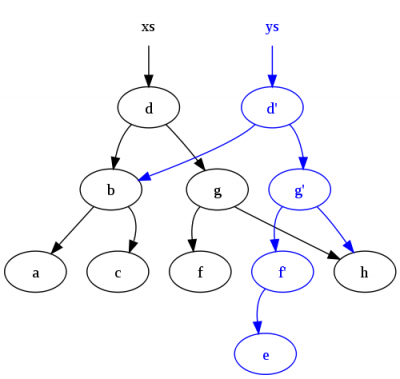
\includegraphics[scale=0.25]{per3.png}
%  \caption{Nondestructive Update}
%  \label{nondesup}
%\end{figure}

%\begin{center}
%\end{center}

%\PSbox{out.ps hscale=25 vscale=25}{0.25in}{0.25in}

\section{Choice of Data Structures}

The chosen data structures provide a wide variety of performance
characteristics and APIs. They include data structures designed for
particular use cases and those that are only performant for certain
operations. These include a variety of single and double-ended queues
(otherwise known as deques), variants of heaps and sets, red-black
trees, treaps, tries and hash lists. Implementing a wide variety of data
structures with the same API allows studying the practical performance
characteristics of each variant, since different variants provide widely
varying running times for specific operations.

%Functional data structures chosen for implementation include functional
%data structures with different performance characteristics, that provide
%different APIs and data structures in which only certain operations are
%performant and hence are suitable only for certain applications. The
%data structures implemented include variants of FIFO queues, variants of
%double ended queues aka deques, variants of lists, variants of heaps,
%variants of sets, red-black tree, treap, tries, and hash list. All the
%variants of the same kind data structure were implemented to study the
%practical performance characteristics of each variant as each variant
%provides different algorithmic running times for its operations.

Another factor influencing the variety of data structures is Typed
Racket. By choosing a wide variety of data structures, each with its own
type invariants and type system requirements, Typed Racket's type system
is exercised and validated in many different ways.

\section{Data Structure Interfaces}

%The library developed to support this thesis consists of more than 25
%distinct data structures.

All the data structures in the library are polymorphic in their element
type and provide utility functions such as \scheme|map|, \scheme|fold|
and \scheme|filter| as well as basic API operations. Each of the queue
implementations share a common API, and similarly for deques, heaps and
other data structures. The following subsections describe the basic
interface of the each category of data structure.

\subsection{Queue Interface}
Queues are First-In-First-Out (FIFO) data structures. All the queue
implementations in the library use the type \scheme|(Queue alpha)|,
where \scheme|alpha| is the polymorphic type variable. Each queue data
structure shares the following common interface:

\begin{file}{Queue Interface}
\begin{schemedisplay}
  ;; Constructs a queue of type \scheme|(Queue alpha)|.
  (: queue : (All (alpha) alpha * -> (Queue alpha))


  ;; Checks if the given queue is empty
  (: empty? : (All (alpha) (Queue alpha) -> Boolean))
  

  ;; Returns the first element of the given queue.
  (: head : (All (alpha) (Queue alpha) -> alpha)


  ;; Returns the tail of the given queue, i.e. a queue without the
  ;; first element of the given queue.
  (: tail : (All (alpha) (Queue alpha) -> (Queue alpha))


  ;; Inserts the given element into the given queue.
  (: enqueue : (All (alpha) alpha (Queue alpha) -> (Queue alpha)))

\end{schemedisplay}
\end{file}

%\vspace{4 mm}

%\scheme|empty?| : \scheme|(All (alpha) (Queue alpha) -> Boolean)|
%\noindent
%\\
%Checks if the given queue is empty.
% 
%\vspace{4 mm}
% 
%\scheme|queue->list| : \scheme|(All (alpha) (Queue alpha) -> (Listof alpha))|
%\noindent
%\\
%Returns a list of all the elements in the given queue. 

%----------------------------------------------------------------


\subsection{Interface for Deque}
Double ended queues are also known as deques. Elements can be inserted
and removed from either end of a deque. The following basic interface
are provided by deque data structure and they have the type
\scheme|(Deque alpha)|:

\begin{file}{Deque Interface}
  \begin{schemedisplay}
    ;; Constructs a deque of type \scheme|(Deque alpha)|.
    (: deque : (All (alpha) alpha * -> (Deque alpha)))

    ;; Checks if the given deque is empty
    (: empty? : (All (alpha) ((Deque alpha) -> Boolean)))

    ;; Returns the first element of the given deque.
    (: head : (All (alpha) (Deque alpha) -> alpha))


    ;; Returns the last element of the given deque.
    (: last : (All (alpha) (Deque alpha) -> alpha))


    ;; Returns the tail of the given deque, i.e. a deque without the first
    ;; element of the given deque.
    (: tail : (All (alpha) (Deque alpha) -> (Deque alpha)))


    ;; Returns a deque without the last element of the given deque.
    (: init : (All (alpha) (Deque alpha) -> (Deque alpha)))


    ;; Inserts the given element to the rear of the given deque.
    (: enqueue : (All (alpha) alpha (Deque alpha) -> (Deque alpha)))


    ;; Inserts the given element to the front of the given deque.
    (: enqueue-front : (All (alpha) alpha (Deque alpha) -> (Deque alpha)))

  \end{schemedisplay}
\end{file}
  
%\vspace{4 mm}
% 
%\scheme|empty?| : \scheme|(All (alpha) (Deque alpha) -> Boolean)|
%\noindent
%\\
%Checks if the given deque is empty.
% 
%\vspace{4 mm}
% 
%\scheme|deque->list| : \scheme|(All (alpha) (Deque alpha) -> (Listof alpha))|
%\noindent
%\\
%Returns a list of all the elements in the given deque.


%\clearpage
\subsection{Heap Interface}

Heaps are tree-based data structures that satisfy two additional
constraints:

\begin{description}
\item[Shape] All its levels of the tree must be full
  except the last level where only rightmost leaves may be missing.
\item[Parental Dominance] The key at each node of the tree
  must greater than or equal (max-heap) OR less than or equal (min-heap)
  to the keys of its children.
%  A tree satisfying this property is said to be \emph{heap-ordered}.
\end{description}
\noindent
All the heaps have the type \scheme|(Heap alpha)|:

\begin{file}{Heap Interface}
  \begin{schemedisplay}

    ;; Constructs a heap with the given elements and 
    ;; \scheme|(alpha alpha -> Boolean)| as its comparison function.
    (: heap : (All (alpha) (alpha alpha -> Boolean) alpha * -> (Heap alpha)))


    ;; Checks if the given heap is empty.
    (: empty? : (All (A) ((Heap A) -> Boolean)))

    
    ;; Inserts the given element into the given heap.
    (: insert : (All (alpha) alpha (Heap alpha) -> (Heap alpha)))


    ;; Returns the min or the max element of the given heap.
    (: find-min/max : (All (alpha) (Heap alpha) -> alpha))


    ;; Deletes the min or the max element of the given heap.
    (: delete-min/max : (All (alpha) (Heap alpha) -> (Heap alpha)))

  \end{schemedisplay}
\end{file}
%\vspace{4 mm}
% 
%\scheme|sorted-list| : \scheme|(All (alpha) (Heap alpha) -> (Listof alpha))|
%\noindent
%\\
%Creates a sorted list of elements out of the elements from the given
%heap sorted with the comparison function of the heap.


\subsection{List Interface}

Alternatives to the Racket's built-in lists. They have the type
\scheme|(List alpha)|\footnote{Typed Racket also provides a built-in
type \scheme|(List alpha)|. The two types can be disambiguated using
Racket's module system.} and provide the following functions:


\begin{file}{List Interface}
  \begin{schemedisplay}
    ;; Constructs a list with the given elements.
    (: list : (All (alpha) alpha * -> (List alpha)))

    ;; Checks if the given list is empty.
    (: empty? : (All (alpha) ((List alpha) -> Boolean)))


    ;; Adds the given element to the front of the given list.
    (: cons : (All (alpha) alpha (List alpha) -> (List alpha)))


    ;; Returns the first element of the given list.
    (: first : (All (alpha) (List alpha) -> alpha))


    ;; Returns the list without the first element of the given list.
    (: rest : (All (alpha) (List alpha) -> (List alpha)))

  \end{schemedisplay}
\end{file}

\subsection*{Random Access List}
Random Access Lists are lists with efficient array-like random access
operations. These include \scheme|list-ref| and \scheme|list-set| (a
functional analogue of \scheme|vector-set!|). Random Access Lists
extend the basic list interface with the following operations:

\begin{file}{RAList Interface}
  \begin{schemedisplay}

    ;; Returns the element at a given location in the list.
    (: list-ref : (All (alpha) Natural (List alpha) -> (List alpha)))


    ;; Updates the element at a given location in the list with a new element.
    (: list-set : (All (alpha) Natural (List alpha) alpha -> (List alpha)))

  \end{schemedisplay}
\end{file}

\subsection*{Catenable List}
Catenable Lists are a list data structure with an efficient append
operation:

\begin{file}{Catenable List Interface}
  \begin{schemedisplay}

    ;; Appends several lists together.
    (: append : (All (alpha) (List alpha) * -> (List alpha))

    
    ;; Inserts a given element to the rear end of the list.
    (: cons-to-end : (All (alpha) alpha (List alpha) -> (List alpha)))

  \end{schemedisplay}
\end{file}
%\vspace{4 mm}



%\vspace{4 mm}
% 
%\scheme|length| : \scheme|(All (alpha) (List alpha) -> Natural)|
%\noindent
%\\
%Returns the length of the given list.


 

%\subsection{Interface for Sets}


%Other data structures include treaps, red-black
%trees, streams and tries. In this chapter, I describe the structure,
%contents of the library, report their performance and compare them with
%imperative data structures.

\section{Data Structure Implementation}

This section describes the theory and performance characteristics of
each data structure in the library.
%and shows example uses of each data structure.

\subsection{Queue Implementations}

\subsection*{Banker's Queue}

Banker's Queues \citep{oka} use a method of amortization known as the
banker's method. Banker's Queues combine lazy evaluation and memoization
to obtain \emph{O}(1) amortized running times for the \scheme|head|,
\scheme|tail| and \scheme|enqueue| operations. The implementation uses
lazy lists to achieve lazy evaluation. The basic structure of Banker's
Queue is similar to the Batched Queue implementation from
Figure~\ref{fig:queueds}. The difference between the two definitions is
that Banker's Queue uses streams as described in Section~\ref{stream}
instead of lists and maintains the invariant \scheme|lenf leq lenr|.

\begin{datastructure}
\begin{schemedisplay}
  langtr

  (struct: (alpha) Queue
    ([front : (Stream alpha)]
     [lenf  : Natural]
     [rear  : (Stream alpha)]
     [lenr  : Natural]))

\end{schemedisplay}
\end{datastructure}

%Banker's Queues provide a amortized running time of \emph{O}(1) .

\subsection*{Physicist's Queue}
\label{phy}
Physicist's Queue \citep{oka} uses a method of amortization called the
physicist's method. The Physicist's Queue also uses lazy evaluation and
memoization to achieve improved amortized running times for its
operations. The only drawback of the physicist's method is that it is
much more complicated than the banker's method.

Unlike Banker's Queues, Physicist's Queues use suspended lists of type
\scheme|(Promise (Listof alpha))| for front instead of streams. Streams
are similar to \scheme|cons|-lists except that every cell in a stream is
delayed. In contrast, suspended lists wrap ordinary \scheme|cons|-lists
in a single delay. The rear is an ordinary list and is not suspended.

The lengths of the lists are explicitly tracked and guaranteed that the
front list is always at least as long as the rear list. Since the front
list is delayed, its first element cannot be accessed without executing
the entire suspension. So, a working copy of a prefix of the front list
is also maintained. This working copy is represented as an ordinary list
for efficient access, and is non-empty whenever the front list is
non-empty. The following box shows the underlying structure of
Physicist's Queue.

\begin{datastructure}
\begin{schemedisplay}
  langtr

  (struct: (alpha) Queue
    ([pref  : (Listof alpha)]
     [front : (Promise (Listof alpha))]
     [lenf  : Natural]
     [rear  : (Listof alpha)]
     [lenr  : Natural]))

\end{schemedisplay}
\end{datastructure}

The Physicist's Queue provides an amortized running time of \emph{O}(1)
for the operations \scheme|head|, \scheme|tail| and
\scheme|enqueue|. The implementation of Physicist's Queue is slightly
complicated than Banker's Queue though they have the same amortized
running times.

\subsection*{Real-Time Queue}
Real-Time Queues eliminate the amortization of the Banker's and
Physicist's Queues to produce a queue with excellent worst-case as well
as amortized running times. Real-Time Queues employ lazy evaluation and
a technique called \emph{scheduling} \citep{oka} where lazy components
are forced systematically so that no suspension takes more than constant
time to execute, assuring good asymptotic worst-case running time for
the operations on the data structure. The structure of Real-Time Queues
differs from Banker's Queues in three ways. First, Real-Time Queues
maintain an extra field of type \scheme|(Stream alpha)| called a
\scheme|schedule|, which determines when \scheme|front| is
forced. Second, Real-Time Queues does not maintain length fields as the
information is available in \scheme|schedule|. And third, \scheme|rear|
is a list and not a stream.

\begin{datastructure}
\begin{schemedisplay}
  langtr
  
  (struct: (alpha) Queue
    ([front      : (Stream alpha)]
     [rear       : (Listof alpha)]
     [schedule : (Stream alpha)]))
\end{schemedisplay}
\end{datastructure}

Unlike Physicist's Queues and Banker's Queues which have a amortized
running times, Real-Time Queues have an \emph{O}(1) worst-case running
time for the operations \scheme|head|, \scheme|tail| and
\scheme|enqueue|.


\subsection*{Implicit Queue}
Implicit Queues implement a queue data structure via \emph{implicit
recursive slowdown} \citep{oka}. Implicit recursive slowdown combines
laziness with a technique called \emph{recursive slowdown} introduced by
\cite{kaplan-tarjan}. This technique is simpler than pure recursive
slow-down, but with the disadvantage of amortized rather than worst-case
bounds on the running time. Similar to Physicist's Queues and Banker's
Queues and unlike Real-Time Queues, Implicit Queues provide an amortized
running time of \emph{O}(1) for the operations \scheme|head|,
\scheme|tail| and \scheme|enqueue|.


\subsection*{Bootstrapped Queue}
The technique of \emph{bootstrapping} is applicable to problems whose
solutions require solutions to simpler instances of the same
problem. Bootstrapped Queues use \emph{structural decomposition}
\citep{oka}.  In structural decomposition, an implementation that can
handle data up to a certain bounded size is used to implement a data
structure that can handle data of unbounded size. Bootstrapped Queues
give a worst-case running time of \emph{O}(1) for the operation
\scheme|head| and \emph{O}(log*~n) for \scheme|tail| and \scheme|enqueue|.
Any queue implementation can be used for bootstrapping. For performance
reasons, my implementation of Bootstrapped Queue uses Physicist's Queue
for bootstrapping.

%\footnote[1]{\emph{log*n} is at most 5 for all feasible queue lengths.}

\subsection*{Hood-Melville Queue}
Hood-Melville Queues \citep{hood-mel} resemble Real-Time Queues in many
ways. Both Real-Time and Hood-Melville Queues maintain two lists front
and rear and incrementally rotate the elements from rear list to front
list when the rear list becomes longer than the front list. The way the
elements are rotated is different. Hood-Melville Queues use a more
complex technique, called \emph{global rebuilding}. In global
rebuilding, reversing of the rear list is done incrementally, a few
steps of reversing per normal operation on the data
structure. Hood-Melville Queues have worst-case running times of
\emph{O}(1) for the operations \scheme|head|, \scheme|tail| and
\scheme|enqueue|.

\subsection{Deque Implementations}

\subsection*{Banker's Deque}
Banker's Deques \cite{oka} are double-ended queues with amortized
running times. They use the banker's method. The structure of Banker's
Deque is similar to the structure of Banker's Queue, using streams and
employing the same techniques used in Banker's Queues to achieve
amortized running times of \emph{O}(1) for the operations \scheme|head|,
\scheme|tail|, \scheme|last|, \scheme|init|, \scheme|enqueue-front| and
\scheme|enqueue|.


\subsection*{Implicit Deque}
The techniques used by Implicit Deques are same as that used in Implicit
Queues i.e., implicit recursive slowdown \citep{oka}. Implicit Deques
provide \emph{O}(1) amortized running times for the operations
\scheme|head|, \scheme|tail|, \scheme|last|, \scheme|init|,
\scheme|enqueue-front| and \scheme|enqueue|.


\subsection*{Real-Time Deque}
Real-Time Deques \citep{oka} eliminate the amortization in the Banker's
Deque to produce deques with good worst-case behavior. The Real-Time
Deques employ the same techniques employed by the Real-Time Queues to
provide worst-case running time of \emph{O}(1) for the operations
\scheme|head|, \scheme|tail|, \scheme|last|, \scheme|init|,
\scheme|enqueue-front| and \scheme|enqueue|.

\subsection{Heap Implementations}

\subsection*{Binomial Heap}
A Binomial Heap \citep{vuillemin, brown} is a heap-ordered binomial
tree. Binomial trees maintains a natural number called its
\emph{rank}. The tree structure is defined as follows:
\begin{itemize}
  \item{A Binomial Tree with rank 0 is a leaf with one element.}

  \item{A Binomial Tree with rank \scheme|r + 1| is composed of two
  trees of rank \scheme|r|.}
\end{itemize}

Binomial Heaps support a fast \scheme|merge| operation using the special
tree structure. Data~Structure~\ref{ds:5} the underlying structure of
Binomial Heaps in Typed Racket.

\begin{datastructure}
  \begin{schemedisplay}

    (struct: (alpha) Node
      ([rank : Natural]
       [elem : alpha]
       [trees : (Listof (Node alpha))]))

    (struct: (alpha) Heap
      ([compare : (alpha alpha -> Boolean)]
       [trees       : (Listof (Node alpha))]))
  \end{schemedisplay}
  \label{ds:5}
\end{datastructure}

\noindent
Binomial Heaps provide a worst-case running time of \emph{O}(log~n) for
the operations \scheme|insert|, \scheme|find-min/max| and
\scheme|delete-min/max|.

\subsection*{Leftist Heap}
Leftist Heaps \citep{crane} are heap-ordered binary trees that satisfy
the \emph{leftist property}.  Each node in the tree is assigned a value
called a \emph{rank}.  The rank represents the length of its rightmost
path from the node in question to the nearest leaf. The leftist property
requires that the right descendant of each node has a lower rank than
the node itself. As a consequence of the leftist property, the right
spine of any node is always the shortest path to a leaf
node. Data~Structure~\ref{ds:6} shows the structure of Leftist Heaps in
Typed Racket.% is:% defined as follows.

\begin{datastructure}
  \begin{schemedisplay}

    (struct: (alpha) Node
      ([rank : Natural]
       [elem : alpha]
       [left   : (Tree alpha)]
       [right : (Tree alpha)]))

    (define-type (Tree alpha) (U Null (Node alpha)))

    (struct: (alpha) Heap
      ([compare : (alpha alpha -> Boolean)]
       [tree        : (Tree alpha)]))

  \end{schemedisplay}
  \label{ds:6}
\end{datastructure}

\noindent
The Leftist Heaps provide a worst-case running time of \emph{O}(log~n)
for the operations \scheme|insert|, \scheme|delete-min/max|,
\scheme|merge| and a worst-case running time of \emph{O}(1) for
\scheme|find-min/max|.

\subsection*{Pairing Heap}
Pairing Heaps \citep{pairing} are a type of heap that simultaneously
have a simple implementation and extremely good amortized performance in
practice. Unfortunately pairing heaps do not cope well with persistence
and hence can be used only in applications that do not take advantage
of persistence.
%However, it has proved very difficult to come up with exact
%asymptotic running time for some operations on Pairing Heaps.
Pairing Heaps are heap-ordered multiway trees represented either as a
empty heap or a pair of an element and a list of pairing
heaps. Data~Structure~\ref{ds:7} shows the structure of Pairing Heaps
in Typed Racket.% is:

\begin{datastructure}
  \begin{schemedisplay}

    (struct: (alpha) Node
      ([elem : alpha]
       [trees : (Listof (Tree alpha))]))

    (define-type (Tree alpha) (U Null (Node alpha)))

    (struct: (alpha) Heap
      ([compare : (alpha alpha -> Boolean)]
       [heap       : (Tree alpha)]))

  \end{schemedisplay}
  \label{ds:7}
\end{datastructure}

\noindent
Pairing Heaps provide a worst-case running time of \emph{O}(1) for the
operations \scheme|insert|, \scheme|find-min/max| and \scheme|merge|,
and an amortized running time of \emph{O}(log~n) for
\scheme|delete-min/max|.

\subsection*{Splay Heap}
Splay Heaps \citep{sla} are similar to balanced binary search trees.
Data~Structure~\ref{ds:8} shows the structure of Splay Heaps in Typed
Racket.
% is:

\begin{datastructure}
  \begin{schemedisplay}

    (struct: (alpha) Node
      ([element : alpha]
       [left        : (Tree alpha)]
       [right      : (Tree alpha)]))

    (define-type (Tree alpha) (U Null (Node alpha)))

    (struct: (alpha) Heap 
      ([compare : (alpha alpha -> Boolean)]
       [heap       : (Tree alpha)]))

  \end{schemedisplay}
  \label{ds:8}
\end{datastructure}

\noindent
The difference between a Splay Heap and a balanced binary search tree is
that Splay Heaps do not maintain explicit balance information. Instead,
every operation on a splay heap restructures the tree with
transformations that increase the balance. Because of the restructuring
on every operation, the worst-case running time of all operations is
\emph{O}(n). However, the amortized running time of the operations
\scheme|insert|, \scheme|find-min/max|, \scheme|delete-min/max| and
\scheme|merge| is \emph{O}(log~n).

\subsection*{Skew Binomial Heap}
Skew Binomial Heaps are similar to Binomial Heaps but with a hybrid
numerical representation for heaps that is based on the \emph{skew
  binary numbers} \citep{skew}. The skew binary number representation is
used since incrementing skew binary numbers is quick and simple. Since
the skew binary numbers have a complicated addition, the \scheme|merge|
operation is based on the ordinary binary numbers itself. Skew Binomial
Heaps provide a worst-case running time of \emph{O}(log~n) for the
operations \scheme|find-min/max|, \scheme|delete-min/max| and
\scheme|merge|, and a worst-case running time of \emph{O}(1) for the
\scheme|insert| operation.

\subsection*{Lazy Pairing Heap}
Lazy Pairing Heaps \citep{oka} are similar to pairing heaps, except that
Lazy Pairing Heaps use lazy evaluation.  Lazy evaluation is used in this
data structure so that the Pairing Heap can cope with persistence
efficiently. Analysis of Lazy Pairing Heaps to obtain exact asymptotic
running times is difficult, as it is for Pairing Heaps. Lazy Pairing
Heaps provide a worst-case running time of \emph{O}(1) for the
operations \scheme|insert|, \scheme|find-min/max|, and \scheme|merge|,
and an amortized running time of \emph{O}(log~n) for the
\scheme|delete-min/max| operation.

\subsection*{Bootstrapped Heap}
Bootstrapped Heaps \citep{oka} use a technique of bootstrapping called
\emph{structural abstraction}, where one data structure abstracts over a
less efficient data structure to get better running times.  Bootstrapped
Heaps provide a worst-case running time of \emph{O}(1) for the
\scheme|insert|, \scheme|find-min/max| and \scheme|merge| operations and
a worst-case running time of \emph{O}(log~n) for \scheme|delete-min/max|
operation. Any heap implementation can be used for bootstrapping. For
practical reasons, my implementation of Bootstrapped Heap abstracts over
Skew Binomial Heaps.

%Due The implementation of Bootstrapped Heap
%abstracts over Skew Binomial Heaps though any other heap implementation
%could be used.

\subsection{List Implementations}
%\subsection*{Random Access List}
%Random Access Lists are lists with efficient array-like random access
%operations. These include \scheme|list-ref| and \scheme|list-set| (a
%functional analogue of \scheme|vector-set!|). Random Access Lists extend
%the basic list interface with \scheme|list-ref| and \scheme|list-set|
%operations.
%\begin{itemlist}
%  \item{\scheme|list-ref : (All (alpha) (List alpha) Integer → alpha)|
%         Returns the element at a given location in the list.}
%  \item{\scheme|list-set : (All (alpha) (List alpha) Integer alpha → (List alpha))|
%    Updates the element at a given location in the list with a new element.}
%)

%\scheme|list-ref : (All (alpha) Natural (List alpha) -> (List alpha))|
%\noindent
%\\
%Returns the element at a given location in the list.
% 
%\vspace{4 mm}
% 
%\scheme|list-set : (All (alpha) Natural (List alpha) alpha -> (List alpha))|
%\noindent
%\\
%Updates the element at a given location in the list with a new element

\subsection*{Binary Random Access List}
Binary Random Access Lists abstract the similarities between
representations of the numbers and lists to derive a representation of
list structure. The Binary Random Access List representation abstracts
over the binary numerical representation \citep{oka} to achieve a
worst-case running time of \emph{O}(log~n) for its random-access
operations \scheme|list-ref| and
\scheme|list-set|. Data~Structure~\ref{ds:9} shows the structure of he
structure of Binary Random Access Lists in Typed Racket.

\begin{datastructure}
  \begin{schemedisplay}

    (struct: (alpha) Leaf ([first : alpha]))

    (struct: (alpha) Node 
      ([first  : alpha]
       [left    : (Tree alpha)] 
       [right : (Tree alpha)]))

    (define-type (Tree alpha) (U (Leaf alpha) (Node alpha)))

    (struct: (alpha) Root 
      ([size  : Integer]
       [first : (Tree alpha)]
       [rest  : (List alpha)]))

    (define-type (List alpha) (U Null (Root alpha)))

  \end{schemedisplay}
  \label{ds:9}
\end{datastructure}

\noindent
Binary Random Access Lists provide a worst-case running time of
\emph{O}(log~n) for the operations \scheme|cons|, \scheme|first| and
\scheme|rest| contrary to Typed Racket's built-in list's worst-case
running time of \emph{O}(1) for the same operations.

\subsection*{Skew Binary Random Access List}
Skew Binary Random Access Lists are similar to Binary Random Access
Lists, but use the skew binary number representation, improving the
running times of some operations. Unlike Binary Random Access Lists,
that have worst-case running time of \emph{O}(log~n), Skew Binary Random
Access Lists provide worst-case running time of \emph{O}(1) for the
operations \scheme|cons|, \scheme|head| and \scheme|tail|. And like
Binary Random Access Lists, Skew Binary Random Access Lists also provide
worst-case running time of \emph{O}(log~n) for \scheme|list-ref| and
\scheme|list-set| operations.

\subsection*{VList}
VLists \citep{bagwell-lists} resemble normal cons lists but provide
efficient versions of many operations that are much slower on standard
lists. They combine the extensibility of linked lists with the fast
random access capability of arrays. Data~Structure~\ref{ds:10} shows the
structure of VLists in Typed Racket. The \scheme|elements| field in the
\scheme|Base| in Data~Structure~\ref{ds:10} is a random access list.
%, along with many other operations,
%some of them are given below.


%\scheme|last| : \scheme|(All (alpha) (List alpha) -> alpha)| \\
%Returns the last element of the given list.
%\vspace{4 mm}
% 
%\scheme|list-ref| : \scheme|(All (alpha) (List alpha) Integer -> alpha)| \\
%Gets the element at the given index in the list.

\begin{datastructure}
  \begin{schemedisplay}
    langtr

    (struct: (alpha) Base
      ([previous : (Block alpha)]
       [elements : (List alpha)]))

    (define-type (Block alpha) (U Null (Base alpha)))

    (struct: (alpha) VList
      ([offset : Integer]
       [base   : (Base alpha)]
       [size    : Integer]))

  \end{schemedisplay}
  \label{ds:10}
\end{datastructure}

\noindent
VLists provide worst-case running times of \emph{O}(1) for the
operations \scheme|cons|, \scheme|head| and \scheme|tail|,
\scheme|list-ref| and \scheme|list-set| operations. This VList
implementation is built internally on Skew Binary Random Access
Lists. VLists provide the standard Random Access List API operations.

\subsection*{Catenable List}
%@subsection[#:tag "catenable"]{Catenable List}
Catenable Lists \citep{catenable} are a list data structure with an
efficient append operation, achieved using the bootstrapping technique
of \emph{structural abstraction}. Catenable Lists are abstracted over
Bootstrapped Queue. They have an amortized running time of \emph{O}(1)
for the basic list operations and for the operations
\scheme|cons-to-end| and \scheme|append|.
%It has the type \scheme|(List alpha)|.

\subsection*{Streams}
\label{stream}
Streams \citep{oka} are also known as lazy lists. They are similar to
ordinary lists and provide a similar API. Stream API provides
\scheme|stream|, \scheme|stream-car|, \scheme|stream-cdr| and
\scheme|stream-cons| which are similar to \scheme|list|, \scheme|first|,
\scheme|rest| and \scheme|cons| from the list interface
respectively. Along with these basic functions, Stream API also provide
some utility functions. Many data structures implemented in this library
use Streams to achieve lazy evaluation. Streams do not change the
asymptotic performance of any list operations, but introduce overhead at
each suspension. And forcing a suspension takes no more than \emph{O}(1)
and hence \scheme|stream-car|, \scheme|stream-cdr| and
\scheme|stream-cons| have a running time of \emph{O}(1). Since streams
have distinct evaluation behavior, they are given a distinct type,
\scheme|(Stream alpha)|.


\subsection{Other Data Structures}
\subsection*{Hash Lists}
Hash Lists \citep{bagwell-lists} are similar to association lists, and
are implemented using a modified VList structure. The modified VList
contains two components: the data and the hash table. Both components
grow as the hash list grows. The running time for Hash Lists operations
such as \scheme|insert|, \scheme|delete|, and \scheme|lookup| are close
to those for standard chained hash tables.

\subsection*{Tries}
A Trie (also known as a Digital Search Tree) \citep{oka} is a data
structure that takes advantage of the structure of aggregate types to
achieve good running times for its operations. Our implementation
provides Tries in which the keys are lists of the element type; this is
sufficient for representing many aggregate data structures. In our
implementation, each trie is a multiway tree with each node of the
multiway tree carrying data of base element type.  Tries provide
\scheme|lookup| and \scheme|insert| operations with better asymptotic
running times than hash tables.

\subsection*{Red-Black Tree}
Red-Black Trees \citep{red-black} are a classic data structure,
consisting of a binary search trees in which every node is colored
either red or black, according to the following two balance invariants:

\begin{itemize}
\item{no red node has a red child, and}
\item{every path from root to an empty node has the same number of black
  nodes.}
\end{itemize}
  
The two invariants together guarantee that the longest possible path
with alternating black and red nodes, is no more then twice as long as
the shortest possible path, with black nodes only. This property helps
achieve good running times for the tree operations. This implementation
is based on \citet{oka-red-black}. Data~Structure~\ref{ds:11} shows the
structure of Red-Black Trees in Typed Racket.

\begin{datastructure}
  \begin{schemedisplay}
    langtr

    (define-type Color (U 'red 'black))
     
    (struct: (alpha) RedBlackNode
      ([color     : Color]
       [element : alpha]
       [left        : (Tree alpha)]
       [right      : (Tree alpha)]))
     
    (define-type (Tree alpha) (U Null (RedBlackNode alpha)))
     
    (struct: (alpha) RedBlackTree
      ([compare : (alpha alpha -> Boolean)]
       [tree        : (Tree alpha)]))

  \end{schemedisplay}
  \label{ds:11}
\end{datastructure}

The operations \scheme|member?|, \scheme|insert| and \scheme|delete|,
which respectively check membership, insert and delete elements from the
tree, have worst-case running time of \emph{O}(log~n). Red-Black Trees
have the type \scheme|(RedBlackTree alpha)|.


\subsection*{Treap}
Treaps \citep{treap} are binary search trees in which each node has both
a search key and a priority. Its keys are sorted in-order and the
priority of each node is lower than the priorities of its
children. Because of these properties, a treap is a binary search tree
for the keys and a heap for its priorities. Assigning random priorities
to the nodes of the treap results in better balance in the treap. Hence
treaps are also known as randomized binary search
trees. Data~Structure~\ref{ds:12} shows the underlying structure of
Treaps in Typed Racket.


\begin{datastructure}
  \begin{schemedisplay}
    langtr

    (struct: (alpha) Node
             ([element : alpha]
              [left        : (Tree alpha)]
              [right      : (Tree alpha)]
              [priority  : Real]))

    (define-type (Tree alpha) (U Null (Node alpha)))

    (struct: (alpha) Treap
             ([compare : (alpha alpha -> Boolean)]
              [tree        : (Tree alpha)]
              [size        : Integer]))

  \end{schemedisplay}
  \label{ds:12}
\end{datastructure}
Treaps implement a worst case running time of \emph{O}(log~n) for the
operations \scheme|insert|, \scheme|find-min/max| and
\scheme|delete-min/max|. A Treap has the type \scheme|(Treap alpha)|.

%Following are the functions implemented by the Red-Black Tree data structure
% 
%@(itemlist 
%  @item{@italic{redblacktree} : 
%         @racketblock[(∀ (A) ((A A → Boolean) A * → 
%                                          (RedBlackTree A)))| 
%         The Red-Black Tree constructor function. Constructs 
%         a red-black tree from the given elements and the
%         comparison function.}
%  @item{@italic{insert} : @racketblock[(∀ (A) (A (RedBlackTree A) → 
%                                                   (RedBlackTree A)))| 
%         @para{Inserts a given element into the red-black tree.}}
%  @item{@italic{root} : \scheme|(∀ (A) ((RedBlackTree A) → A))| 
%         @para{Returns the root element of the given red-black tree.}}
%  @item{@italic{member?} : @racketblock[(∀ (A) (A (RedBlackTree A) → Boolean))| 
%         Checks if the given element is a member of the 
%         red-black tree.}
%  @item{@italic{delete} : @racketblock[(∀ (A) (A (RedBlackTree A) → 
%                                                   (RedBlackTree A)))| 
%         @para{Deletes the given element from the given red-black 
%         tree.}})

  

%\clearpage
